% For a two-column report, figure* spans both columns.
% Requires \usepackage{graphicx}.
\begin{figure*}[t]
    \centering
    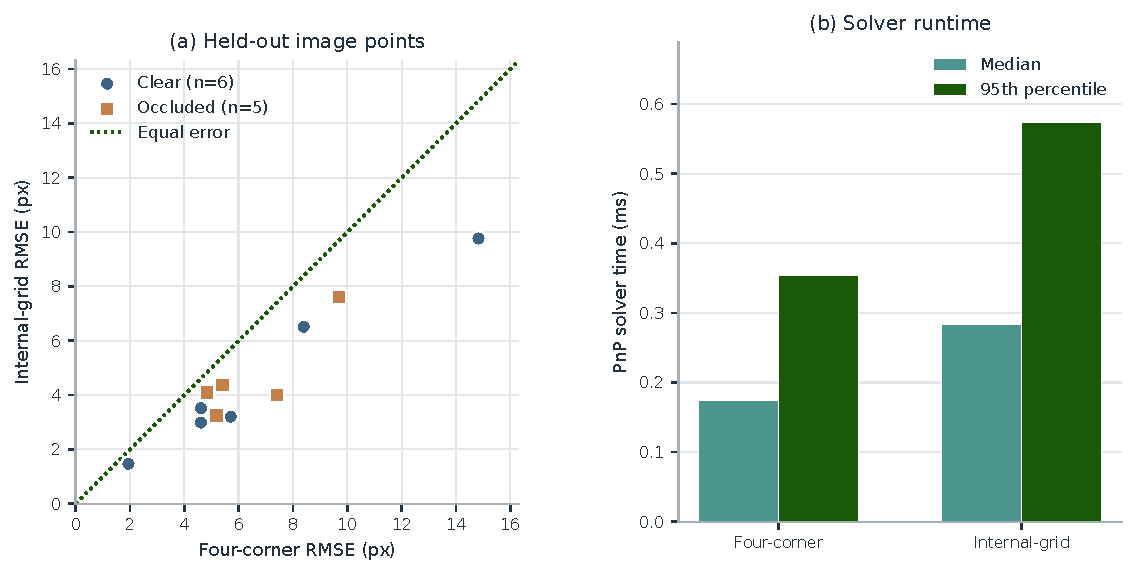
\includegraphics[width=0.88\textwidth]{pose_benchmark/figures/report/pose_results_combined.pdf}
    \caption{(a) Paired manual reprojection RMSE for photographs with valid tracked geometry; the dotted line indicates equal error. (b) Median and 95th-percentile PnP solver times across eligible video frames.}
    \label{fig:pose_comparison}
\end{figure*}

\begin{figure}[t]
    \centering
    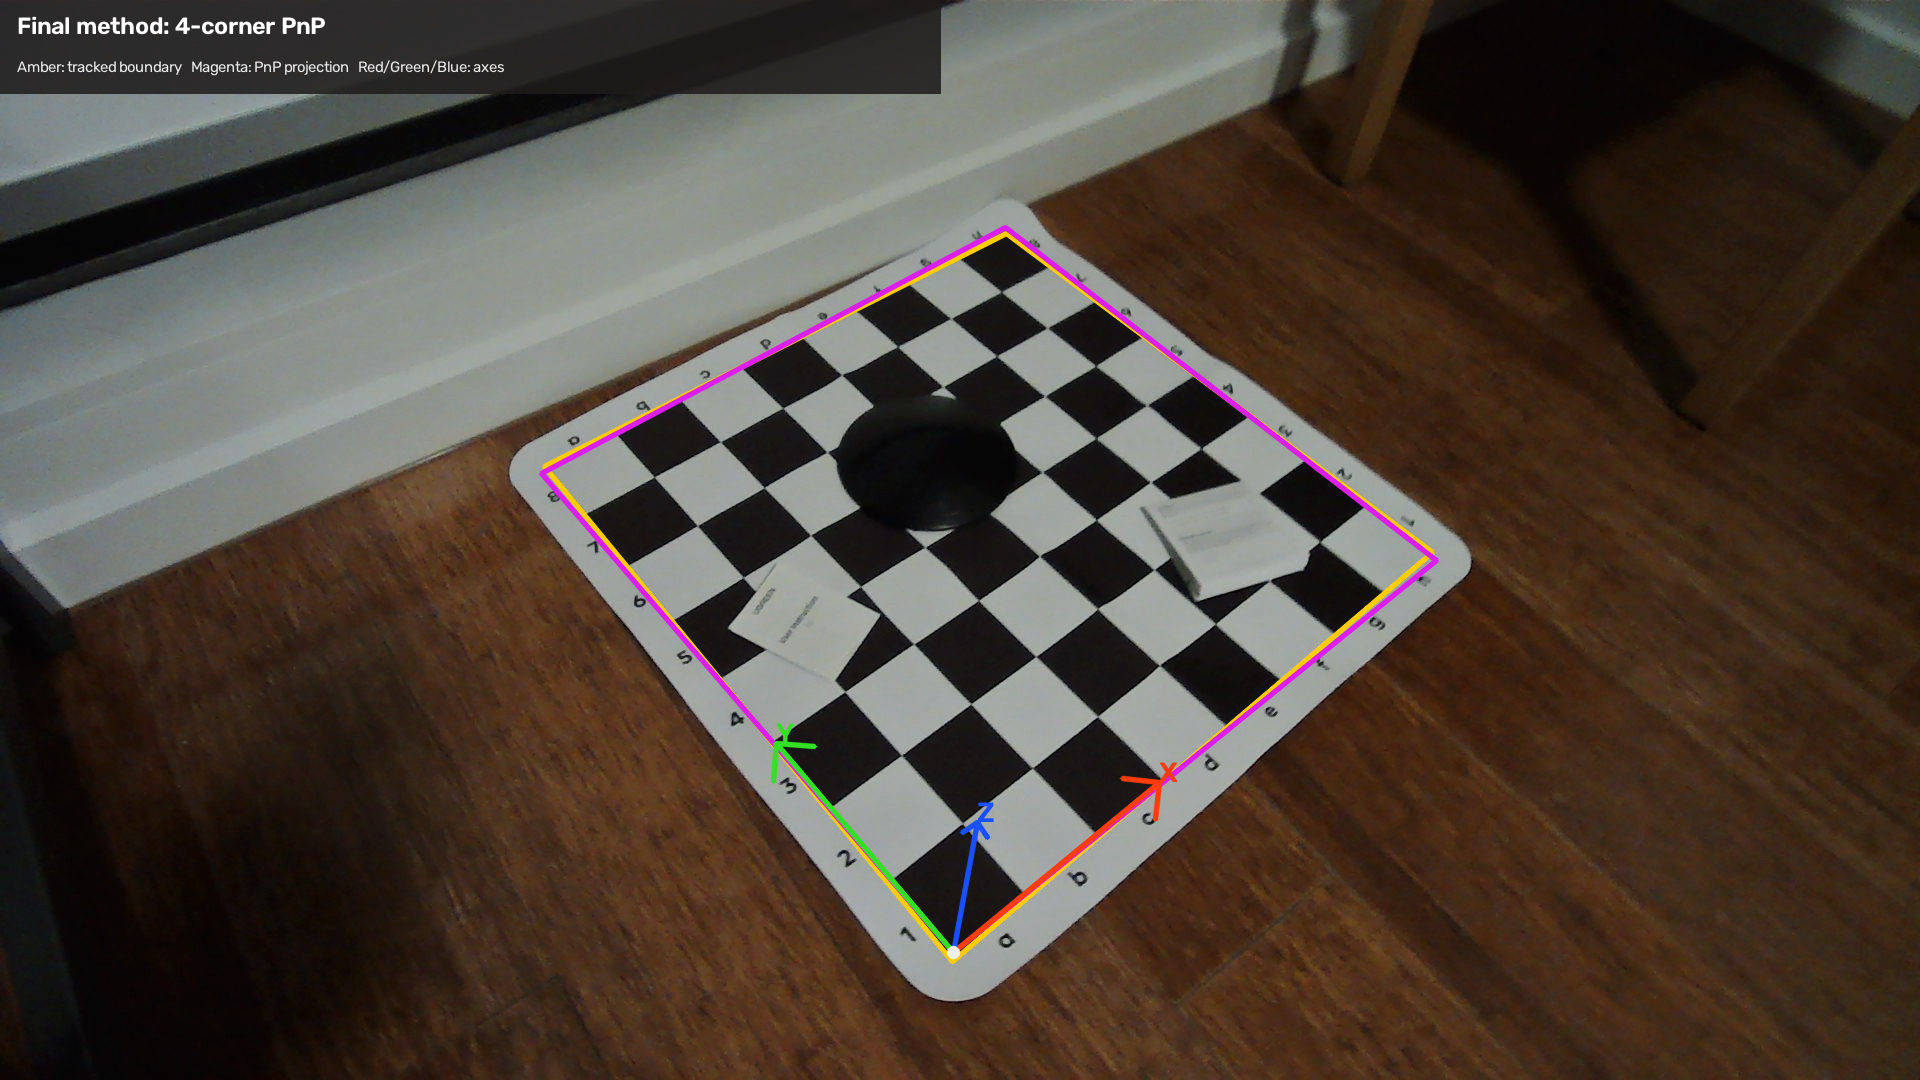
\includegraphics[width=\columnwidth]{pose_benchmark/figures/report/pose_example_four_corner.png}
    \caption{Four-corner PnP pose overlaid on a representative webcam photograph. Amber shows the tracked board boundary, magenta the pose-projected board boundary, and red, green and blue the projected axes at the fixed board origin.}
    \label{fig:pose_example}
\end{figure}
